\begin{figure}[H]
	\centering
	\caption{Steady State $ k^{*} $ at $ c_{t} = c^{*} $}
	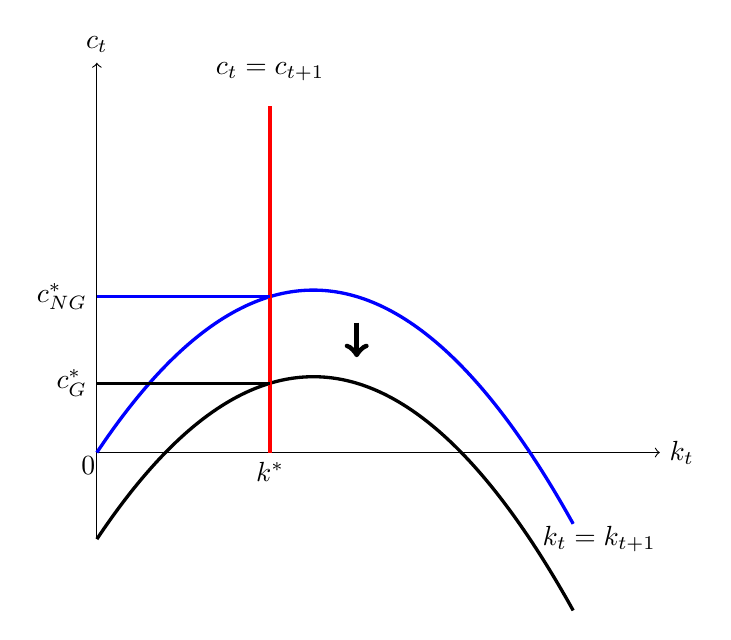
\begin{tikzpicture}[scale=1.1]
		\draw[->] (0, 0) -- (6.5, 0) node[right] {$k_{t}$};
		\draw[->] (0, -1) -- (0, 4.5) node[above] {$c_{t}$};
		\draw[domain=0:5.5, samples=200, blue, line width = 1.2pt, variable=\x] plot ({\x}, {-0.3*\x*(\x-5)});
		\draw[domain=0:5.5, samples=200, black, line width = 1.2pt, variable=\x] plot ({\x}, {-0.3*\x*(\x-5) - 1});
		\draw[red, line width=1.5pt] (2,0) -- (2,4);
		\draw[black, line width=1pt] (2,0.8) -- (0,0.8);
		\draw[blue, line width=1pt] (2,1.8) -- (0,1.8);
		\node at (-0.1,-0.15) {$0$};
		\node at (5.8,-1) {$ k_{t} = k_{t+1} $};
		\node at (2,4.4) {$c_{t} = c_{t+1}$};
		\node[below] at (2,0) {$k^*$};
		\node[left] at (0,0.8) {$c^{*}_{G}$};
		\node[left] at (0,1.8) {$c^{*}_{NG}$};
		\draw[->, line width=2pt] (3,1.5) -- (3,1.1);
	\end{tikzpicture}
\end{figure}
